\documentclass{article}
\usepackage{graphicx}
\usepackage{geometry}
 \geometry{
 a4paper,
 total={170mm,257mm},
 left=20mm,
 top=20mm,
 }
\usepackage{caption}
\usepackage{subcaption}
\usepackage{hyperref}
\graphicspath{{./figs/}}{}
\usepackage{listings}
\title{
HLS-Assignment 9 (PART-1) 
}
\begin{document}
\maketitle
\hfill \textbf{Sampath Govardhan} \\
\null \hfill \textbf{FWC22071}\\
\maketitle
\hfill \textbf{VITIS-HLS}
\section{Problem Statement}
\href{run:./problem_statement.pdf} {Problem Statemt}
\begin{lstlisting}
Design a digital circuit using RTL and HLS for a 5G NR CRC bits generator.

 Requirements: 
1. The module should process 8 bits per clock cycle.
2. The input and output buses should use the AXIS interface.
3. Implement a pipelined design.
4. The implementation should use as minimum resources as possible.

 Considerations:
1. Implement the module only for CRC24A
2. A last signal should be used to indicate the end of the input bit stream.
3. The design implementation should be targeted on the ZCU111 FPGA board.
\end{lstlisting}
\vspace{1cm}
\section{Header File}
\vspace{1cm}
\begin{figure}[h]
\centering
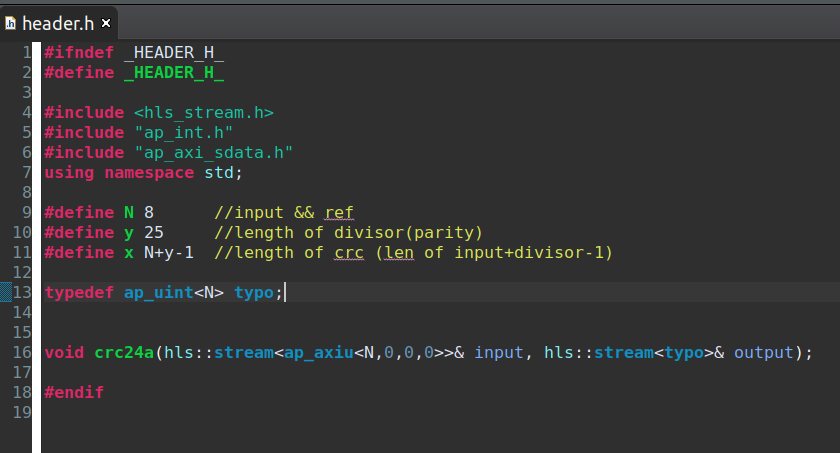
\includegraphics[width=0.8\textwidth]{figs/p1header.png}
    \caption{header.h}
    \label{fig:my_label}
\end{figure}

\vspace{15cm}
\section{Crc bits Generator Code}
\vspace{1cm}
\begin{figure}[h]
\centering
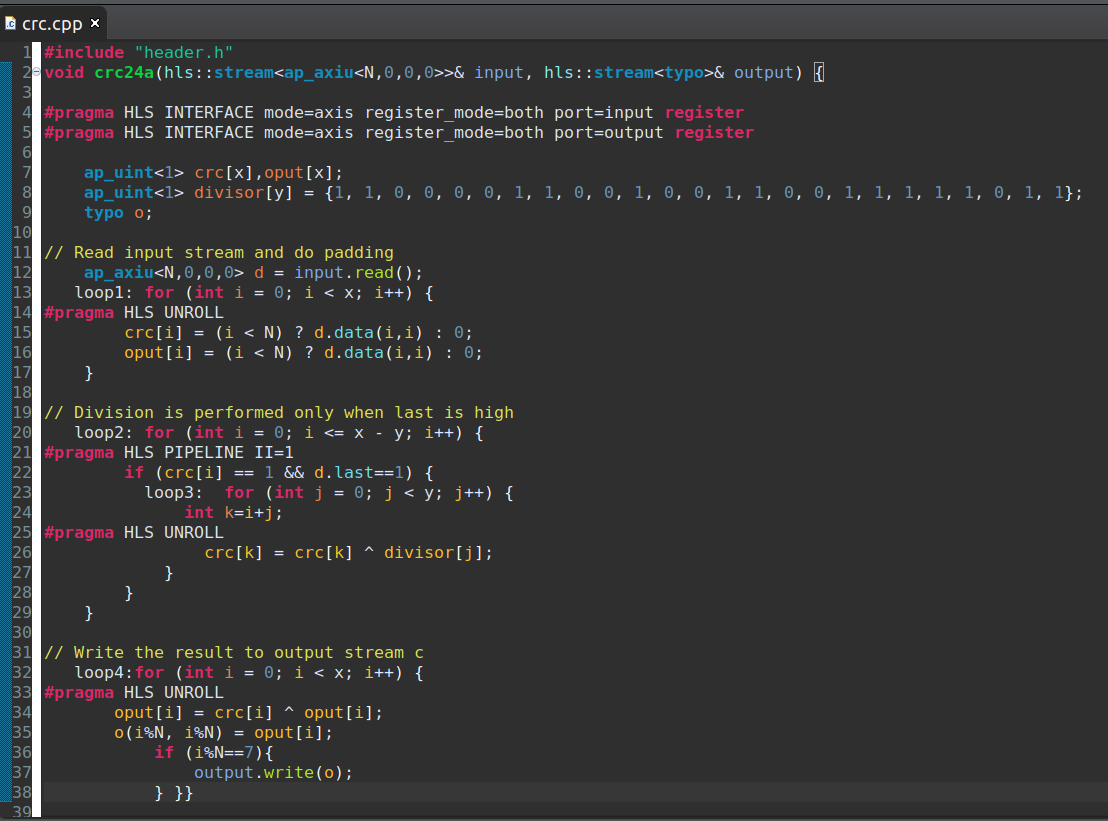
\includegraphics[width=1.1\textwidth]{figs/p1crc.png}
    \caption{crc.cpp}
    \label{fig:my_label}
\end{figure}
\vspace{1cm}
\section{Design Choices}
\begin{lstlisting}

1. I Considered input message of length 8 and I designed the module accordingly.

2. The function takes two parameters: input and output.

   input is an AXIS input stream of ap_axiu type with a width of 8 bits and with 
  a last signal.
  
   output is an AXIS output stream of ap_uint<8> type, since last signal
  is not requested.

3. The pragmas specify the interface properties for the function. mode=axis
  indicates that the function uses an AXI-Stream interface. register_mode=both
  specifies that both the input and output streams should be implemented using
  registers.

4. divisor is an array of ap_uint<1> type with a size of 25(crc24a).

   crc and oput are arrays of ap_uint<1> type with a size of 
  x(input length + divisor length - 1). crc array is used for crc computation 
  and oput array is used to stream output data along with input message.
  
   o is a variable of type ap_uint<8> which is used for storing of output data 
  and then streaming accordingly.
  
   d is a variable of type ap_uint<8> which reads input data. Since I had only
  8 bits input data I read it only once.

5. loop1 initializes values to the crc and oput arrays based on the data present
  in d(from the input stream). It copies the i-th bit of d.data to crc[i] and
  oput[i] and it assigns all other indexes to zero. 
  
    The loop is unrolled to improve the efficiency of copying bits from d.data
  to crc and oput arrays. Unrolling eliminates loop control overhead and allows 
  multiple assignments to be performed in parallel.
  
6. loop2 and loop3 performs the division operation for the CRC algorithm.
  It checks if the i-th bit of crc is 1 and if d.last is also 1 (indicating 
  it is the last element of the input stream). If both conditions are satisfied,
  it performs the XOR operation between crc[k] and divisor[j] and stores the 
  result in crc[k] , where k iterates from i to i+y-1. At the end of loop3 crc 
  array is loaded with crc computed values(remainder) of input message and divisor.
  
   For the loop2 the #pragma HLS PIPELINE II=1 directive is used to pipeline the 
  loop iterations. By applying pipelining, the tool can overlap the execution of 
  consecutive iterations, allowing the operations within the loop to be executed 
  concurrently. This can result in increased throughput.
  
   Additionally, the #pragma HLS UNROLL directive is used for loop3. It  
  instructs the tool to unroll the inner loop completely and multiple loop 
  iterations are executed in parallel, which can further improve parallelism and 
  increase performance.

7. loop4 performs the final XOR operation between crc(has crc computation 
  output) and oput(has input message) arrays(since we need the output in form of 
  input+crcoutput) and updates the o object with the XOR result.
   The line o(i%N, i%N) = oput[i]; assigns the i-th bit of oput to the 
   corresponding position in o. Finally, if the current index i is a multiple of
   8 (i.e., i%N == 7), it writes the o object to the output stream.

   This loop performs the final XOR operation between crc and oput arrays and 
  updates the variable o. Unrolling the loop helps increase parallelism and 
  pipeline the operations for better performance.

8. Overall, this code reads an input stream of AXI-Stream elements and performs
  the CRC-24 algorithm on the data, and writes the result to the output stream.

\end{lstlisting}
\vspace{13cm}

\section{Testbench Code}
\vspace{1cm}
\begin{figure}[h]
\centering
\begin{subfigure}[b]{\textwidth}
    \centering
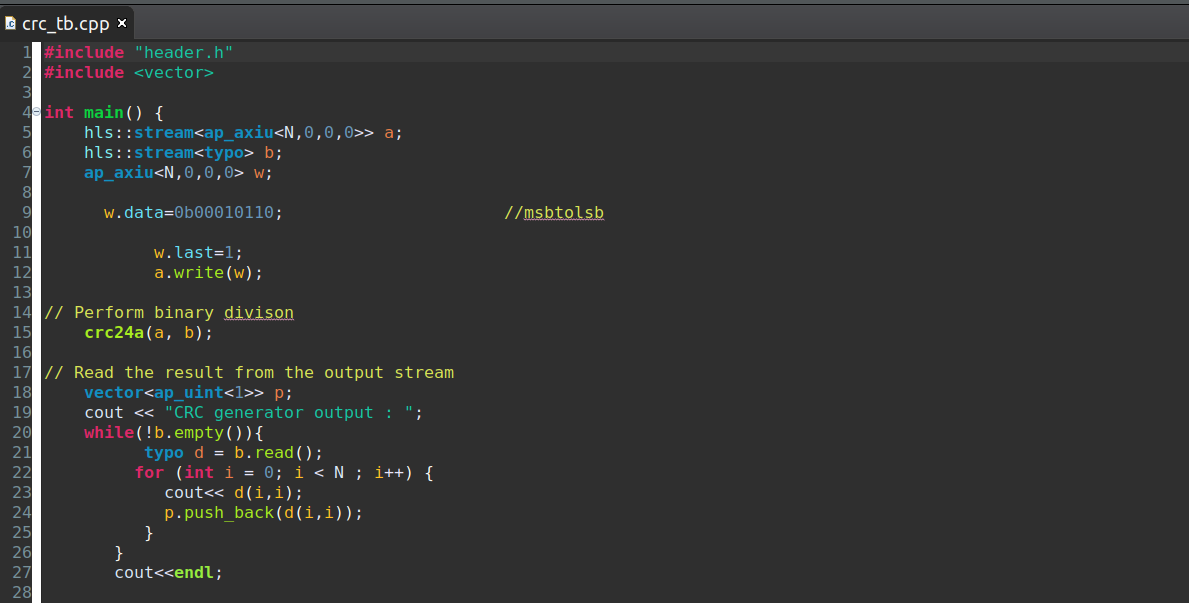
\includegraphics[width=1.1\textwidth]{figs/p1crc_tb1.png}
    \label{fig:my_label}
\end{subfigure}
\hfill
\begin{subfigure}[b]{\textwidth}
    \centering
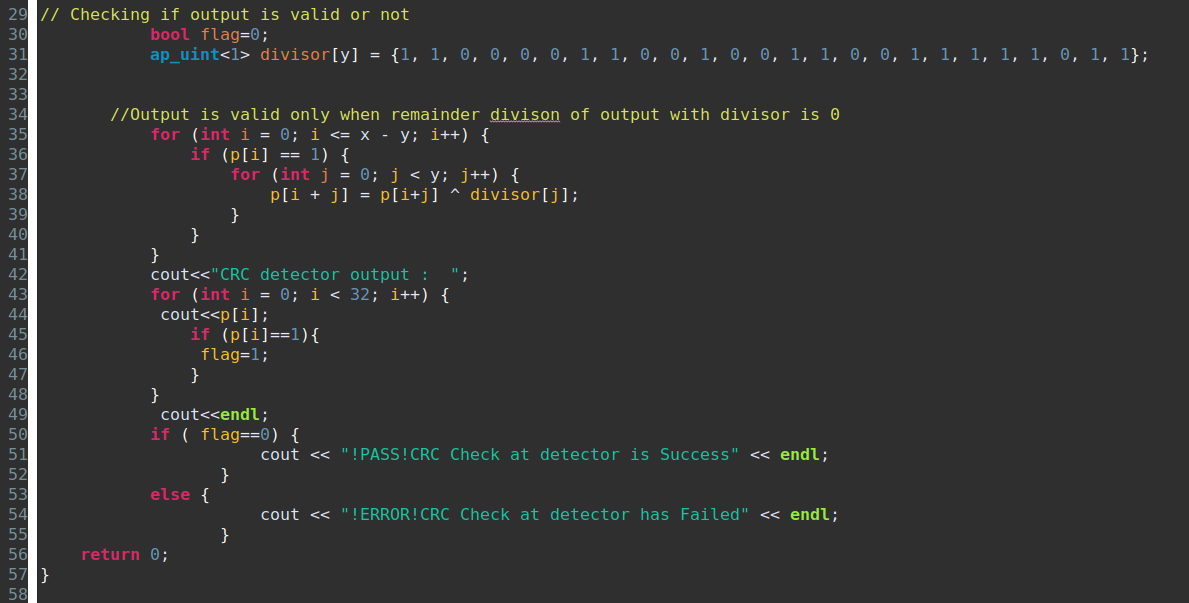
\includegraphics[width=1.1\textwidth]{figs/p1crc_tb2.png}
    \caption{crctb.cpp}
    \label{fig:my_label}
\end{subfigure}
\end{figure}
\vspace{10cm}

\section{C simulation Output}

\begin{figure}[h]
\centering
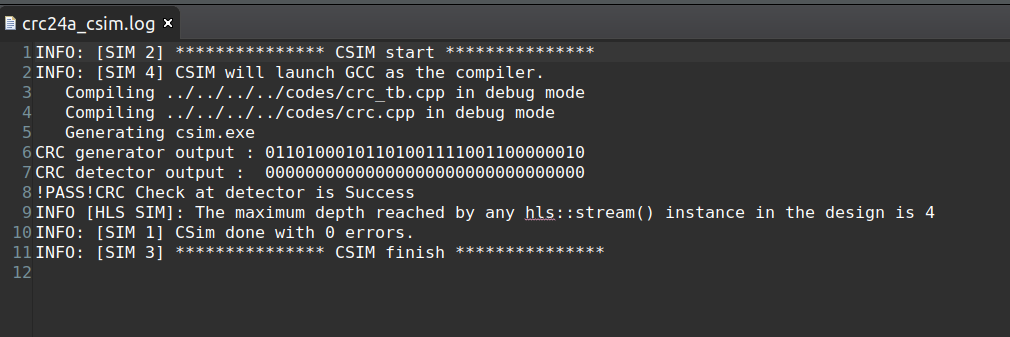
\includegraphics[width=1.1\textwidth]{figs/p1csim.png}
    \caption{C Simulation Output}
    \label{fig:my_label}
\end{figure}
\vspace{1cm}

\section{HLS Resource Consumption Report}
\vspace{1cm}
\begin{figure}[h]
\centering
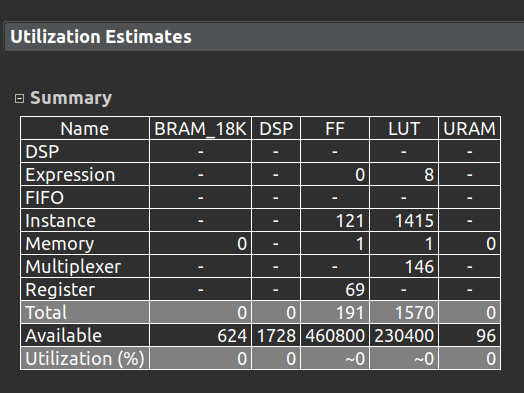
\includegraphics[width=0.8\textwidth]{figs/p11.png}
    \caption{Resource Consumption}
    \label{fig:my_label}
\end{figure}

\vspace{12cm}


\section{HLS Timing and Fmax Report}
\vspace{1cm}
\begin{figure}[h]
    \centering
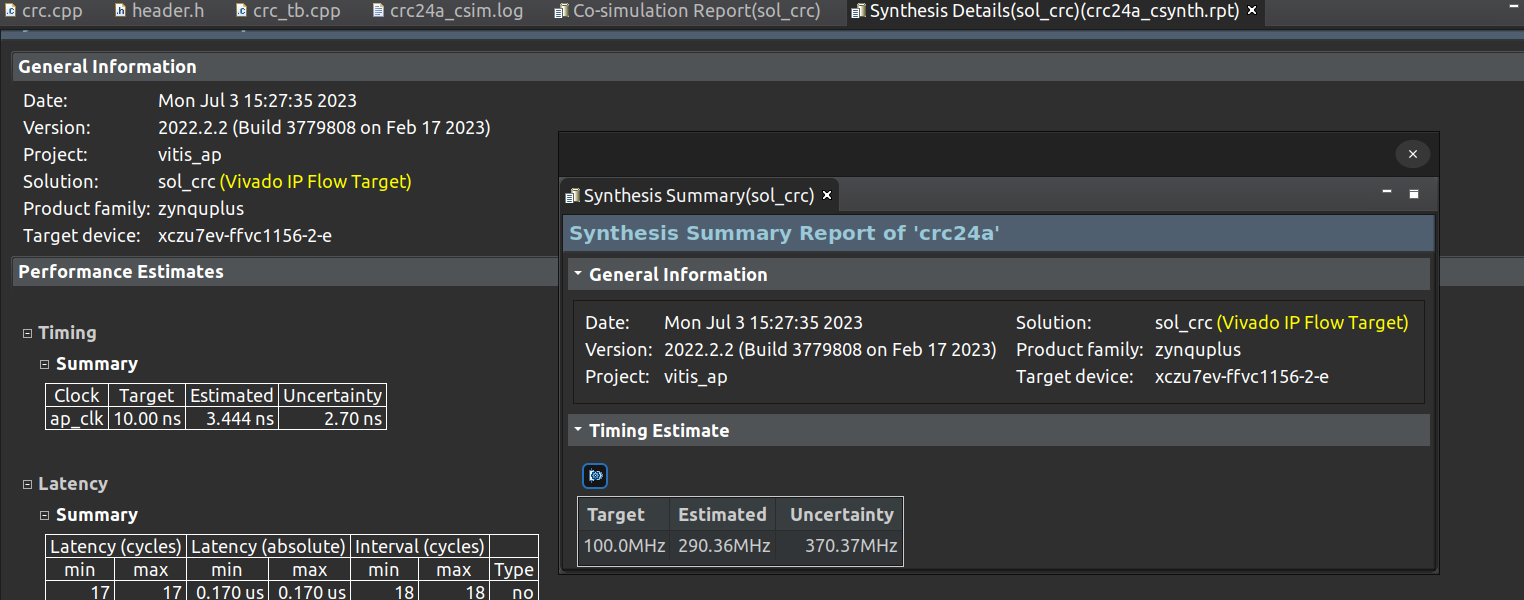
\includegraphics[width=1.1\textwidth]{figs/p12.png}
    \caption{Timing and Fmax}
    \label{fig:my_label}
\end{figure}

\vspace{1cm}


\section{CoSimulation Report}
\vspace{1cm}
\begin{figure}[h]
    \centering
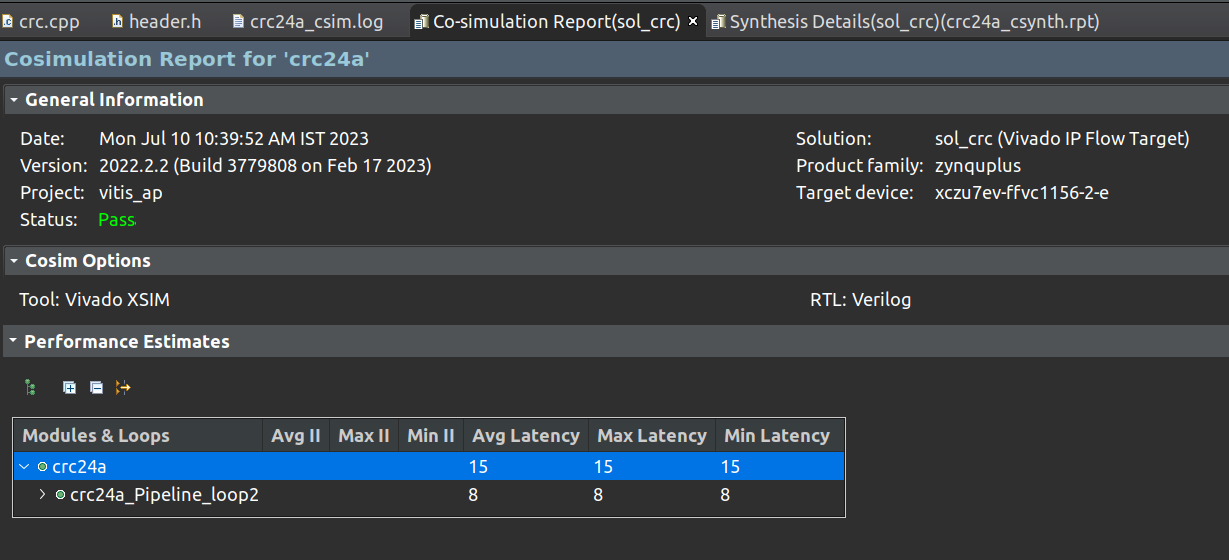
\includegraphics[width=1.1\textwidth]{figs/p13.png}
    \caption{Cosimulation}
    \label{fig:my_label}
\end{figure}

\vspace{15cm}


\section{Performance Evaluation}
\begin{lstlisting}

After synthesis source code has :
  1. Execution Time:          12.65 seconds
  2. Latency:                 16 
  3. Resource Utilization:    87 FF & 875 LUT
  4. Memory Usage:            76.434 MB
  5. Fmax:                    290.36 MHz
  6. Iteration Interval:      17
  7. Throughput:              0.632
 

\end{lstlisting}
\vspace{1cm}


\maketitle
\hfill \textbf{VIVADO}
\section{Block Design}
\vspace{1cm}
\begin{figure}[h]
    \centering
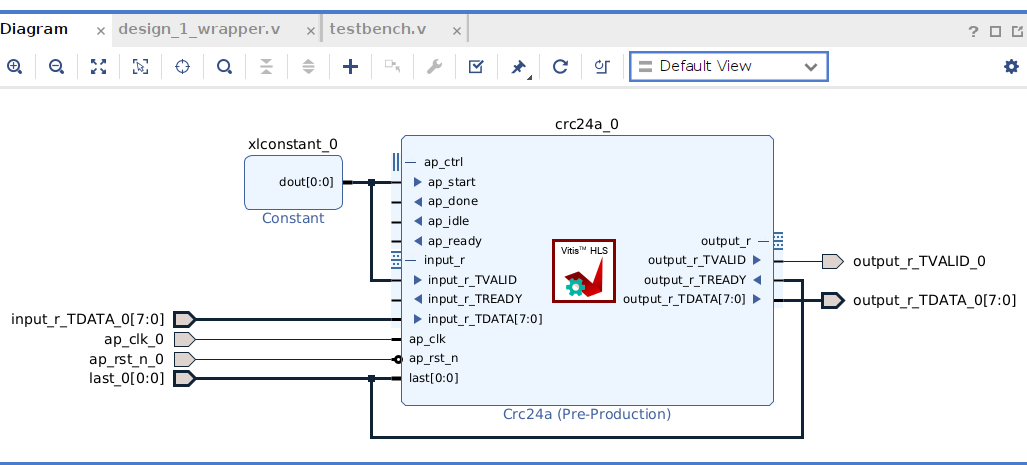
\includegraphics[width=\columnwidth]{figs/p1bd.png}
    \caption{Block Diagram}
    \label{fig:my_label}
\end{figure}
\vspace{13cm}

\section{Verilog Testbench}
\begin{lstlisting}

//testbench.v
`timescale 1ns / 1ps
//////////////////////////////////////////////////////////////////////////////////
// Company: 
// Engineer: 
// 
// Create Date: 06/26/2023 11:35:30 AM
// Design Name: 
// Module Name: testbench
// Project Name: 
// Target Devices: 
// Tool Versions: 
// Description: 
// 
// Dependencies: 
// 
// Revision:
// Revision 0.01 - File Created
// Additional Comments:
// 
//////////////////////////////////////////////////////////////////////////////////


module testbench();
        reg ap_clk_0;
        reg ap_rst_n_0;         
        reg [7:0] ip;
        reg input_r_TLAST_0;  
        wire [7:0] op;
        wire output_r_TVALID_0;
        
        
   design_1_wrapper uut(.ap_clk_0(ap_clk_0),.input_r_TLAST_0(input_r_TLAST_0),
   .ap_rst_n_0(ap_rst_n_0),.input_r_TDATA_0(ip),.output_r_TDATA_0(op),
   .output_r_TVALID_0(output_r_TVALID_0));
    
        always #5 ap_clk_0=~ap_clk_0;
        
        initial begin
        ap_clk_0=0;ap_rst_n_0=0;
        #10
        ap_rst_n_0=1;
        #10
        ip=8'b00010110;//ascii "h"
        input_r_TLAST_0=1;
        #180
        $finish;
        end
      
    
endmodule

\end{lstlisting}

\vspace{13cm}


\section{Output Waveform}
\vspace{1cm}
\begin{figure}[h]
\centering
\begin{subfigure}[b]{0.8\textwidth}
    \centering
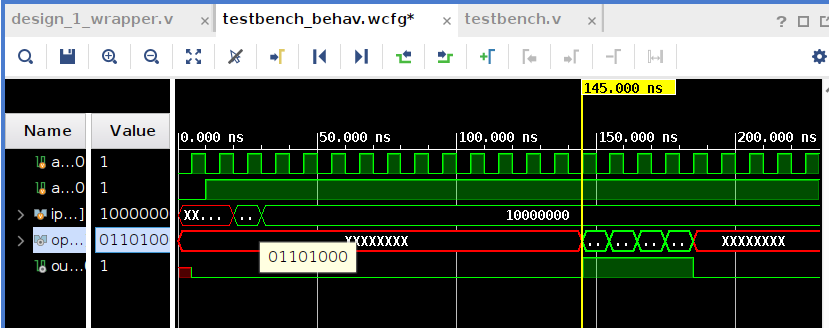
\includegraphics[width=\textwidth]{figs/p1wavfull.png}
    \caption{Output of IP}
    \label{fig:my_label}
\end{subfigure}
\hfill
\begin{subfigure}[b]{0.8\textwidth}
    \centering
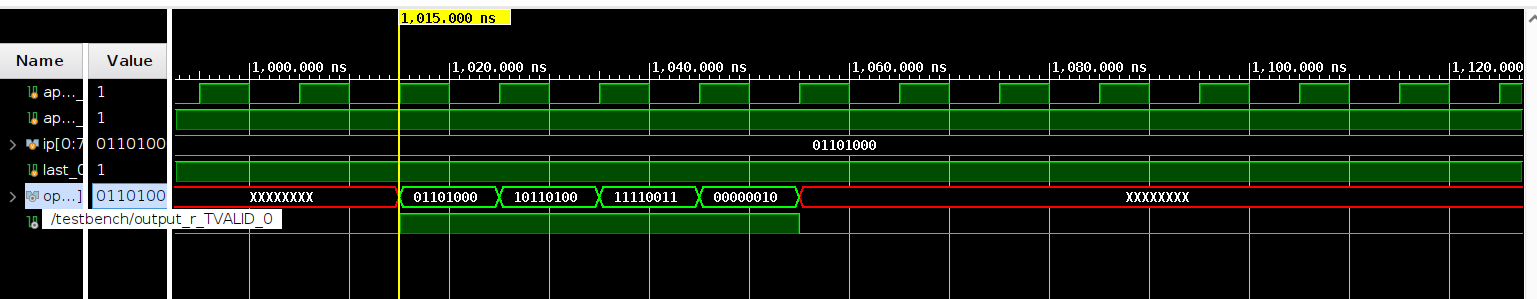
\includegraphics[width=\textwidth]{figs/p1wav.png}
    \caption{Zoomed format of above figure}
    \label{fig:my_label}
\end{subfigure}
\end{figure}


\end{document}


